\chapter{Modes of working}
\label{modes}

\section{Command scripts}
\label{scripts}

As you execute commands in \app{gretl}, using the GUI and filling in
dialog entries, those commands are recorded in the form of a
``script'' or batch file.  Such scripts can be edited and re-run,
using either \app{gretl} or the command-line client, \app{gretlcli}.

To view the current state of the script at any point in a \app{gretl}
session, choose ``Command log'' under the Tools menu. This log
file is called \verb+session.inp+ and it is overwritten whenever you
start a new session.  To preserve it, save the script under a
different name.  Script files will be found most easily, using the GUI
file selector, if you name them with the extension ``\verb+.inp+''.

To open a script you have written independently, use the ``File,
Script files'' menu item; to create a script from scratch use the
``File, Script files, New script'' item or the ``new script'' toolbar
button.  In either case a script window will open (see Figure
\ref{fig-scriptwin}).

\begin{figure}[htbp]
  \begin{center}
    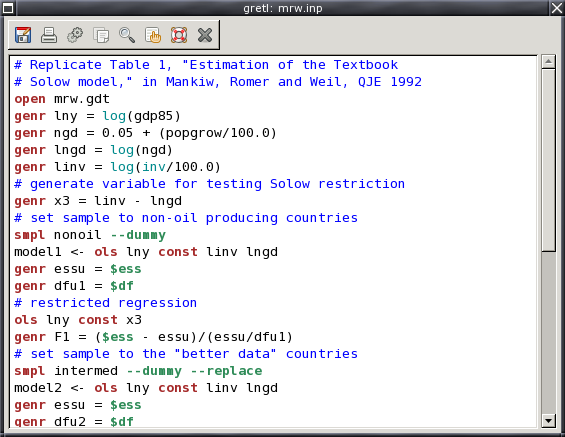
\includegraphics[scale=0.5]{figures/scriptwin}
  \end{center}
  \caption{Script window, editing a command file}
  \label{fig-scriptwin}
\end{figure}

The toolbar at the top of the script window offers the following
functions (left to right): (1) Save the file; (2) Save the file under
a specified name; (3) Print the file (this option is not available on
all platforms); (4) Execute the commands in the file; (5) Copy
selected text; (6) Paste the selected text; (7) Find and replace text;
(8) Undo the last Paste or Replace action; (9) Help (if you place the
cursor in a command word and press the question mark you will get help
on that command); (10) Close the window.

When you execute the script, by clicking on the Execute icon or by
pressing Ctrl-r, all output is directed to a single window, where it
can be edited, saved or copied to the clipboard.  To learn more about
the possibilities of scripting, take a look at the \app{gretl} Help
item ``Command reference,'' or start up the command-line program
\app{gretlcli} and consult its help, or consult the \GCR.

If you run the script when part of it is highlighted, \app{gretl} will
only run that portion. Moreover, if you want to run just the current
line, you can do so by pressing Ctrl-Enter.\footnote{This feature is
  not unique to \app{gretl}; other econometric packages offer the same
  facility. However, experience shows that while this can be
  remarkably useful, it can also lead to writing dinosaur scripts that
  are never meant to be executed all at once, but rather used as a
  chaotic repository to cherry-pick snippets from. Since \app{gretl}
  allows you to have several script windows open at the same time, you
  may want to keep your scripts tidy and reasonably small.}

Clicking the right mouse button in the script editor window produces a
pop-up menu.  This gives you the option of executing either the line
on which the cursor is located, or the selected region of the script
if there's a selection in place.  If the script is editable, this menu
also gives the option of adding or removing comment markers from the
start of the line or lines.

The \app{gretl} package includes over 70 ``practice'' scripts.  Most
of these relate to \cite{ramanathan02}, but they may also be used as a
free-standing introduction to scripting in \app{gretl} and to various
points of econometric theory.  You can explore the practice files
under ``File, Script files, Practice file'' There you will find a
listing of the files along with a brief description of the points they
illustrate and the data they employ.  Open any file and run it to see
the output.  Note that long commands in a script can be broken over
two or more lines, using backslash as a continuation character.

You can, if you wish, use the GUI controls and the scripting approach
in tandem, exploiting each method where it offers greater convenience.
Here are two suggestions.

\begin{itemize}
\item Open a data file in the GUI.  Explore the data --- generate
  graphs, run regressions, perform tests.  Then open the Command log,
  edit out any redundant commands, and save it under a specific name.
  Run the script to generate a single file containing a concise record
  of your work.
\item Start by establishing a new script file.  Type in any commands
  that may be required to set up transformations of the data (see the
  \cmd{genr} command in the \GCR). Typically this sort of thing can be
  accomplished more efficiently via commands assembled with
  forethought rather than point-and-click. Then save and run the
  script: the GUI data window will be updated accordingly.  Now you
  can carry out further exploration of the data via the GUI.  To
  revisit the data at a later point, open and rerun the
  ``preparatory'' script first.
\end{itemize}

\subsection{Scripts and data files}

One common way of doing econometric research with \app{gretl} is as
follows: compose a script; execute the script; inspect the output;
modify the script; run it again --- with the last three steps repeated
as many times as necessary.  In this context, note that when you open
a data file this clears out most of \app{gretl}'s internal state.
It's therefore probably a good idea to have your script start with an
\texttt{open} command: the data file will be re-opened each time, and
you can be confident you're getting ``fresh'' results.

One further point should be noted.  When you go to open a new data
file via the graphical interface, you are always prompted: opening a
new data file will lose any unsaved work, do you really want to do
this?  When you execute a script that opens a data file, however, you
are \textit{not} prompted.  The assumption is that in this case you're
not going to lose any work, because the work is embodied in the script
itself (and it would be annoying to be prompted at each iteration of
the work cycle described above).   

This means you should be careful if you've done work using the
graphical interface and then decide to run a script: the current data
file will be replaced without any questions asked, and it's your
responsibility to save any changes to your data first.


\section{Saving script objects}
\label{sect-script-objects}

When you estimate a model using point-and-click, the model results are
displayed in a separate window, offering menus which let you perform
tests, draw graphs, save data from the model, and so on.  Ordinarily,
when you estimate a model using a script you just get a
non-interactive printout of the results.  You can, however, arrange
for models estimated in a script to be ``captured'', so that you can
examine them interactively when the script is finished.  Here is an
example of the syntax for achieving this effect:
    
\begin{code}
Model1 <- ols Ct 0 Yt
\end{code}
That is, you type a name for the model to be saved under, then a
back-pointing ``assignment arrow'', then the model command.  You may
use names that have embedded spaces if you like, but such names must
be wrapped in double quotes:
\begin{code}
"Model 1" <- ols Ct 0 Yt
\end{code}
Models saved in this way will appear as icons in the \app{gretl}
icon view window (see Section \ref{session}) after the script is
executed.  In addition, you can arrange to have a named model
displayed (in its own window) automatically as follows:
\begin{code}
Model1.show
\end{code}
Again, if the name contains spaces it must be quoted:
\begin{code}
"Model 1".show
\end{code}
The same facility can be used for graphs.  For example the following
will create a plot of \verb+Ct+ against \verb+Yt+, save it under the
name ``CrossPlot'' (it will appear under this name in the icon
view window), and have it displayed:
\begin{code}
CrossPlot <- gnuplot Ct Yt
CrossPlot.show
\end{code}
You can also save the output from selected commands as named pieces of
text (again, these will appear in the session icon window, from where
you can open them later).  For example this command sends the output
from an augmented Dickey--Fuller test to a ``text object'' named
\verb+ADF1+ and displays it in a window:
\begin{code}
ADF1 <- adf 2 x1
ADF1.show
\end{code}
Objects saved in this way (whether models, graphs or pieces of text
output) can be destroyed using the command \verb+.free+ appended to
the name of the object, as in \verb+ADF1.free+.

\section{The gretl console}
\label{console}

A further option is available for your computing convenience. Under
\app{gretl}'s ``Tools'' menu you will find the item ``Gretl console''
(there is also an ``open gretl console'' button on the toolbar in the
main window).  This opens up a window in which you can type commands
and execute them one by one (by pressing the Enter key) interactively.
This is essentially the same as \app{gretlcli}'s mode of operation,
except that the GUI is updated based on commands executed from the
console, enabling you to work back and forth as you wish.

In the console, you have ``command history''; that is, you can use the
up and down arrow keys to navigate the list of command you have
entered to date.  You can retrieve, edit and then re-enter a previous
command.

In console mode, you can create, display and free objects (models,
graphs or text) aa described above for script mode.

\section{The Session concept}
\label{session}

\app{gretl} offers the idea of a ``session'' as a way of keeping track
of your work and revisiting it later. The basic idea is to provide an
iconic space containing various objects pertaining to your current
working session (see Figure \ref{fig-session}).  You can add objects
(represented by icons) to this space as you go along.  If you save the
session, these added objects should be available again if you re-open
the session later.

\begin{figure}[htbp]
  \begin{center}
    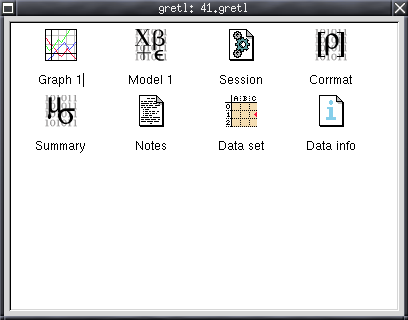
\includegraphics[scale=0.5]{figures/session}
  \end{center}
  \caption{Icon view: one model and one graph have been added to the
    default icons}
  \label{fig-session}
\end{figure}

If you start \app{gretl} and open a data set, then select ``Icon
view'' from the View menu, you should see the basic default set of
icons: these give you quick access to information on the data set (if
any), correlation matrix (``Correlations'') and descriptive summary
statistics (``Summary''). All of these are activated by
double-clicking the relevant icon.  The ``Data set'' icon is a little
more complex: double-clicking opens up the data in the built-in
spreadsheet, but you can also right-click on the icon for a menu of
other actions.

To add a model to the Icon view, first estimate it using the Model
menu.  Then pull down the File menu in the model window and select
``Save to session as icon\dots{}'' or ``Save as icon and close''.
Simply hitting the \verb+S+ key over the model window is a shortcut to
the latter action.

To add a graph, first create it (under the View menu, ``Graph
specified vars'', or via one of \app{gretl}'s other graph-generating
commands).  Click on the graph window to bring up the graph menu, and
select ``Save to session as icon''.

Once a model or graph is added its icon will appear in the Icon view
window.  Double-clicking on the icon redisplays the object, while
right-clicking brings up a menu which lets you display or delete the
object.  This popup menu also gives you the option of editing graphs.

\subsection{The model table}
\label{model-table}

In econometric research it is common to estimate several models with a
common dependent variable --- the models differing in respect of which
independent variables are included, or perhaps in respect of the
estimator used.  In this situation it is convenient to present the
regression results in the form of a table, where each column contains
the results (coefficient estimates and standard errors) for a given
model, and each row contains the estimates for a given variable across
the models.  

In the Icon view window \app{gretl} provides a means of constructing
such a table (and copying it in plain text, {\LaTeX} or Rich Text
Format).  The procedure is outlined below.  (The model table can also
be built non-interactively, in script mode.  For details, see the
entry for \cmd{modeltab} in the \emph{Gretl Command Reference}.)

      
\begin{enumerate}
\item Estimate a model which you wish to include in the table, and in
  the model display window, under the File menu, select ``Save to
  session as icon'' or ``Save as icon and close''.
\item Repeat step 1 for the other models to be included in the table
  (up to a total of six models).
\item When you are done estimating the models, open the icon view of
  your gretl session, by selecting ``Icon view'' under the View
  menu in the main gretl window, or by clicking the ``session icon
  view'' icon on the gretl toolbar.
\item In the Icon view, there is an icon labeled ``Model table''.
  Decide which model you wish to appear in the left-most column of the
  model table and add it to the table, either by dragging its icon
  onto the Model table icon, or by right-clicking on the model icon
  and selecting ``Add to model table'' from the pop-up menu.
\item Repeat step 4 for the other models you wish to include in the
  table.  The second model selected will appear in the second column
  from the left, and so on.
\item When you are finished composing the model table, display it by
  double-clicking on its icon.  Under the Edit menu in the window
  which appears, you have the option of copying the table to the
  clipboard in various formats.
\item If the ordering of the models in the table is not what you
  wanted, right-click on the model table icon and select ``Clear
  table''.  Then go back to step 4 above and try again.
\end{enumerate}

A simple instance of \app{gretl}'s model table is shown in
Figure~\ref{fig-model-table}.

\begin{figure}[htbp]
  \begin{center}
    
\includegraphics[scale=0.5]{figures/model_table}
  \end{center}
  \caption{Example of model table}
  \label{fig-model-table}
\end{figure}


\subsection{The graph page}
\label{sect-graphpage}

The ``graph page'' icon in the session window offers a means of
putting together several graphs for printing on a single page.  This
facility will work only if you have the {\LaTeX} typesetting system
installed, and are able to generate and view either PDF or PostScript
output.  The output format is controlled by your choice of program for
compiling \TeX\ files, which can be found under the ``Programs'' tab
in the Preferences dialog box (under the ``Tools'' menu in the main
window).  Usually this should be \app{pdflatex} for PDF output or
\app{latex} for PostScript.  In the latter case you must have
a working set-up for handling PostScript, which will
usually include \app{dvips}, \app{ghostscript} and a viewer such
as \app{gv}, \app{ggv} or \app{kghostview}.  

In the Icon view window, you can drag up to eight graphs onto the
graph page icon.  When you double-click on the icon (or right-click
and select ``Display''), a page containing the selected graphs (in PDF
or EPS format) will be composed and opened in your viewer.  From there
you should be able to print the page.

To clear the graph page, right-click on its icon and select ``Clear''.

As with the model table, it is also possible to manipulate the graph
page via commands in script or console mode --- see the entry for the
\cmd{graphpg} command in the \emph{Gretl Command Reference}.


\subsection{Saving and re-opening sessions}
\label{session-save}

If you create models or graphs that you think you may wish to
re-examine later, then before quitting \app{gretl} select ``Session
files, Save session'' from the File menu and give a name under
which to save the session.  To re-open the session later, either

\begin{itemize}
\item Start \app{gretl} then re-open the session file by going to the
  ``File, Session files, Open session'', or
\item From the command line, type \cmd{gretl -r} \textsl{sessionfile},
  where \textsl{sessionfile} is the name under which the session was
  saved, or
\item Drag the icon representing a \app{gretl} session file onto
  \app{gretl}.
\end{itemize}


%%% Local Variables: 
%%% mode: latex
%%% TeX-master: "gretl-guide"
%%% End: 

